\section{Results}
\label{sec:results}

\subsection{Authorship is almost perfectly readable}

\begin{table}[t]
\centering
\caption{Held-out authorship readout and direction geometry. Both checkpoints select layer 5 by validation AUROC. Bold marks the best value within each metric; ties are both bolded. Cosines use same-checkpoint directions.}
\label{tab:readout}
\resizebox{\textwidth}{!}{%
\begin{tabular}{@{}lccccccc@{}}
\toprule
\textbf{Checkpoint} & \textbf{Layer} & \textbf{Val. AUROC} & \textbf{Test AUROC} & \textbf{Test acc.} & $\cos(\mathrm{AI},\mathrm{Asst.})$ & $\cos(\mathrm{AI},\mathrm{Form.})$ & $\cos(\mathrm{Asst.},\mathrm{Form.})$ \\
\midrule
\qweninst & 5 / 28 & 0.9991 & \textbf{0.9997} & \textbf{0.9813} & $-0.021$ & $+0.062$ & $+0.827$ \\
\qwenbase & 5 / 28 & \textbf{0.9992} & \textbf{0.9997} & \textbf{0.9813} & $-0.015$ & $-0.046$ & $+0.645$ \\
\bottomrule
\end{tabular}%
}
\end{table}



The validation-selected layer is layer 5 for both checkpoints. It reaches 0.9997 held-out AUROC and 0.9813 accuracy in each case (\tabref{tab:readout}). Readout is not confined to the selected layer: all five tested layers achieve 0.9997--1.000 test AUROC. Under this within-checkpoint design, instruction tuning does not measurably amplify separability. Because the directions are fit separately in each checkpoint, this comparison establishes representational availability, not vector identity across models.

The authorship direction is nearly orthogonal to the measured nuisance axes. In the instruct model, $\cos(\mathrm{AI},\mathrm{Assistant})=-0.021$ and $\cos(\mathrm{AI},\mathrm{formality})=0.062$; the corresponding base-model values are $-0.015$ and $-0.046$. By contrast, Assistant and formality overlap strongly (0.827 instruct; 0.645 base). The raw separator is therefore not simply either nuisance axis under these operationalizations.

\subsection{Writing along the direction does not produce a consistent detector response}

\begin{table}[t]
\centering
\caption{Primary raw-direction endpoint effects ($\alpha=+2$ minus $-2$). Confidence intervals use 5,000 prompt-cluster bootstrap samples; $p$-values use 20,000 paired sign flips. No interval excludes zero, and all Holm-adjusted detector $p$-values equal 1.0.}
\label{tab:causal-effects}
\resizebox{\textwidth}{!}{%
\begin{tabular}{@{}llrrrrr@{}}
\toprule
\textbf{Checkpoint} & \textbf{Outcome} & \textbf{$n$} & \textbf{Mean difference} & \textbf{95\% CI} & \textbf{$\dz$} & \textbf{Perm. $p$} \\
\midrule
\qweninst & \mage $P(\mathrm{AI})$ & 16 & $+0.008$ & $[-0.077,+0.095]$ & $+0.043$ & .864 \\
\qweninst & Public \publicdet $P(\mathrm{AI})$ & 16 & $-0.077$ & $[-0.246,+0.057]$ & $-0.241$ & .390 \\
\midrule
\qwenbase & \mage $P(\mathrm{AI})$ & 12 & $+0.032$ & $[-0.020,+0.088]$ & $+0.323$ & .294 \\
\qwenbase & Public \publicdet $P(\mathrm{AI})$ & 12 & $+0.033$ & $[-0.061,+0.172]$ & $+0.147$ & .874 \\
\bottomrule
\end{tabular}%
}
\end{table}



\Tabref{tab:causal-effects} reports the primary endpoint tests. On the 16 instruct prompts, moving from $\alpha=-2$ to $+2$ changes the \mage detector's $\pa$ by $+0.008$ (95\% CI $[-0.077,0.095]$, $\dz=0.043$, $p=.864$). The public detector moves in the opposite direction: $-0.077$ ($[-0.246,0.057]$, $\dz=-0.241$, $p=.390$). The 12-prompt base replication yields small positive point estimates, but both intervals again cross zero. Every Holm-adjusted detector $p$-value is 1.0.

\begin{figure}[t]
\centering
\begin{subfigure}[b]{0.49\textwidth}
    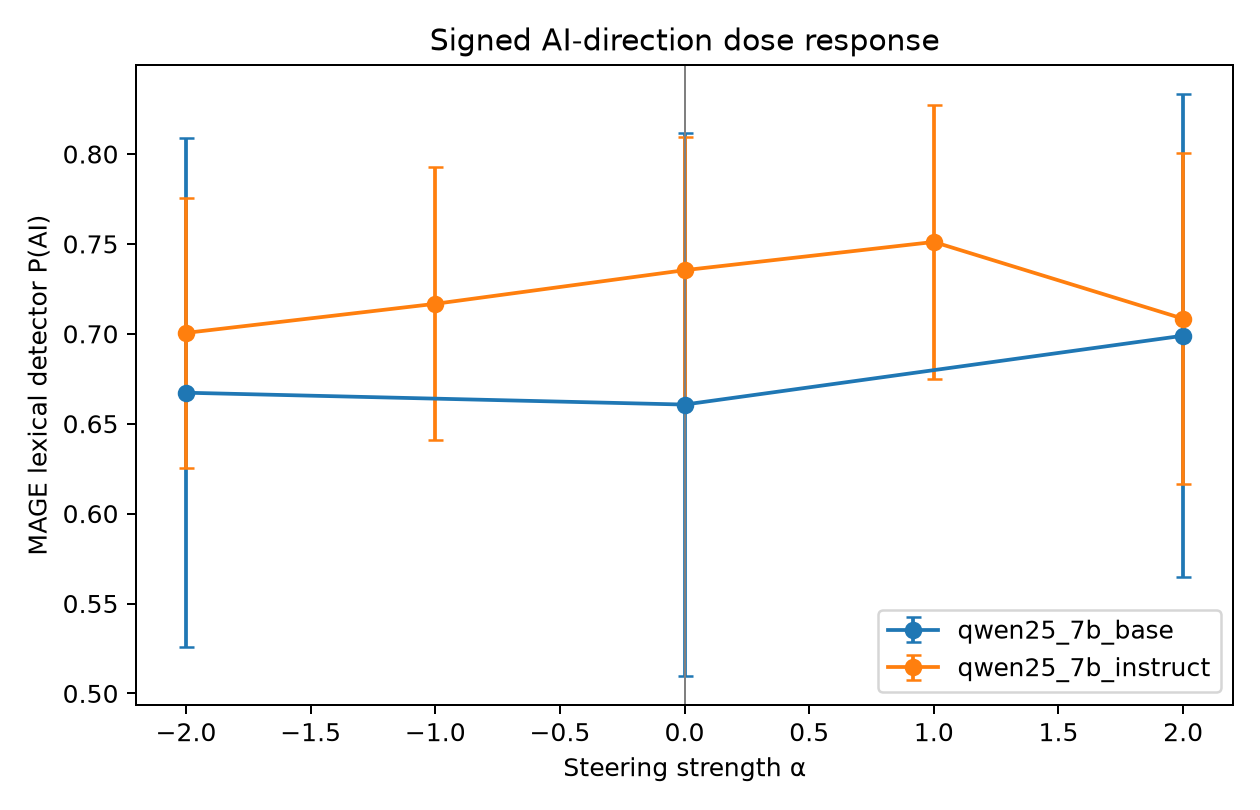
\includegraphics[width=\linewidth]{figures/dose_response_detector_ai.png}
    \caption{\mage-trained TF--IDF detector.}
    \label{fig:dose-mage}
\end{subfigure}
\hfill
\begin{subfigure}[b]{0.49\textwidth}
    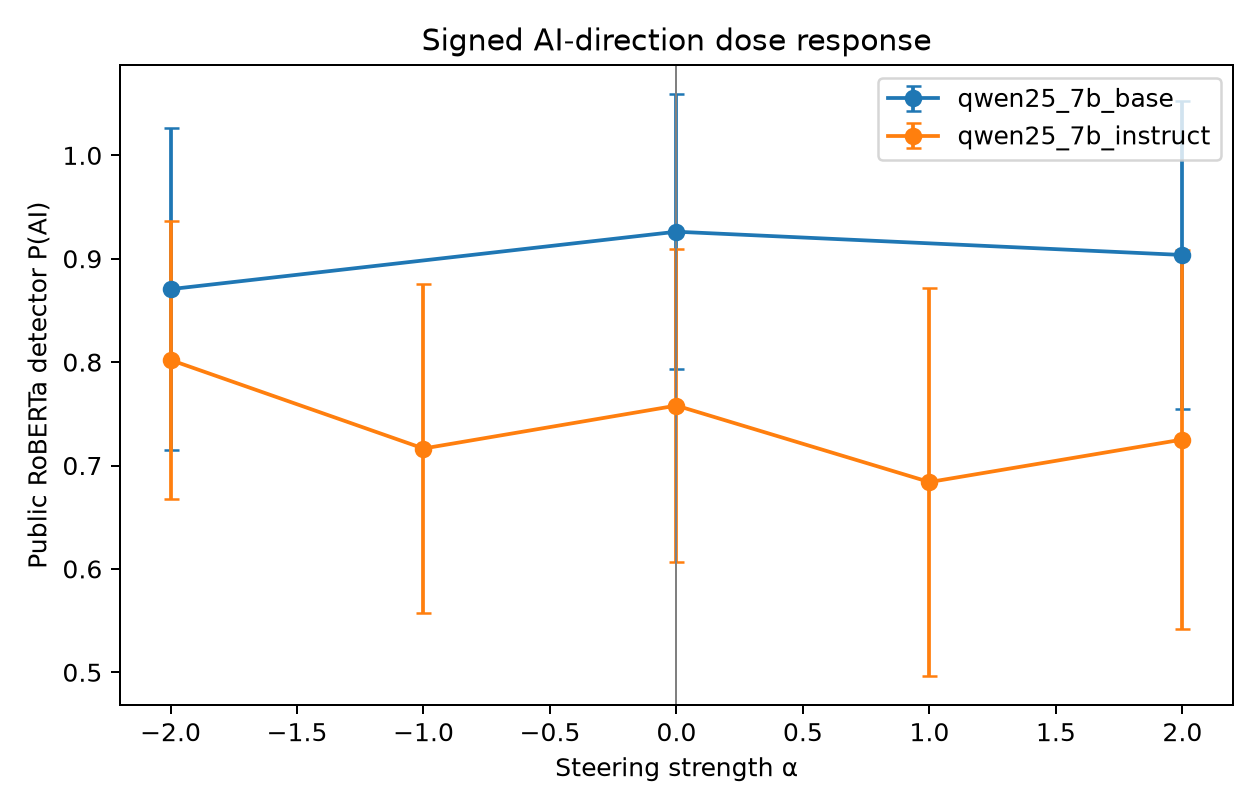
\includegraphics[width=\linewidth]{figures/dose_response_public_detector_ai.png}
    \caption{Public \publicdet detector.}
    \label{fig:dose-public}
\end{subfigure}
\caption{Signed dose response for the raw authorship direction. Points aggregate scores at each dose; uncertainty is computed over prompts. The instruct-model mean within-prompt slopes are $+0.0050$ $P(\mathrm{AI})/\alpha$ (95\% CI $[-0.0122,0.0234]$) for \mage and $-0.0186$ ($[-0.0707,0.0247]$) for \publicdet. Neither detector shows a robust monotonic response, and their slope signs disagree.}
\label{fig:dose-response}
\end{figure}

The full instruct sweep leads to the same conclusion (\figref{fig:dose-response}). Mean within-prompt slopes are $+0.0050$ $P(\mathrm{AI})/\alpha$ ($[-0.0122,0.0234]$) for the \mage detector and $-0.0186$ ($[-0.0707,0.0247]$) for the public detector. Descriptive correlations over the five dose means are $\rho=0.40$ and $\rho=-0.50$, respectively, neither significant. Thus, the data show neither a robust dose response nor agreement between independent measures.

\subsection{Residualization and matched controls do not reveal specificity}

\begin{figure}[t]
\centering
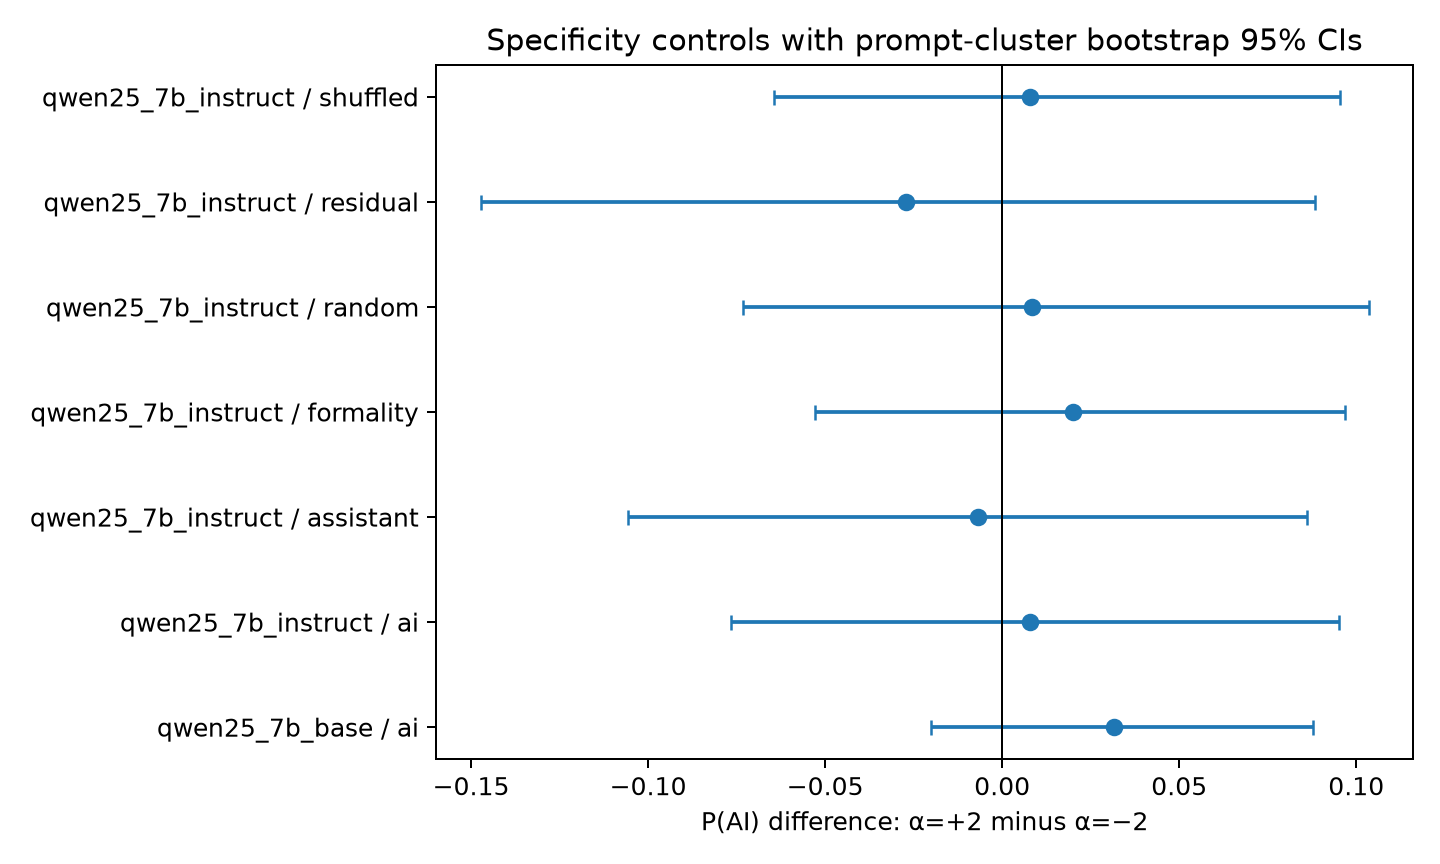
\includegraphics[width=0.95\linewidth]{figures/control_effects.png}
\caption{Endpoint effects ($\alpha=+2$ minus $-2$) for the instruct checkpoint. Error bars are 95\% prompt-cluster bootstrap intervals. All detector intervals cross zero for the raw, nuisance-residualized, random, shuffled-label, formality, and Assistant directions. The raw authorship vector does not outperform equal-norm controls.}
\label{fig:controls}
\end{figure}

For the \mage detector, endpoint differences are $-0.027$ ($[-0.147,0.088]$) for the fully nuisance-orthogonal direction, $+0.008$ ($[-0.073,0.103]$) for the random direction, $+0.008$ ($[-0.064,0.096]$) for shuffled labels, $+0.020$ ($[-0.053,0.097]$) for formality, and $-0.007$ ($[-0.106,0.086]$) for the Assistant axis. Public-detector intervals also all cross zero (\figref{fig:controls}). Removing the measured nuisance span therefore does not uncover a hidden effect, and the raw vector has no demonstrated specificity over matched controls.

\subsection{Endpoint quality does not explain the null}

\begin{table}[t]
\centering
\caption{Quality and preservation changes for the raw instruct direction ($\alpha=+2$ minus $-2$, $n=16$). No 95\% prompt-cluster bootstrap interval excludes zero. Similarity is measured against the same prompt's unsteered continuation.}
\label{tab:quality}
\begin{tabular}{@{}lrr@{}}
\toprule
\textbf{Measure} & \textbf{Mean difference} & \textbf{95\% CI} \\
\midrule
Word count & $+3.19$ & $[-2.19,+8.63]$ \\
Repeated 3-gram rate & $-0.049$ & $[-0.119,+0.010]$ \\
Semantic similarity & $+0.002$ & $[-0.076,+0.078]$ \\
Base-Qwen perplexity & $-6.58$ & $[-19.94,+1.18]$ \\
\bottomrule
\end{tabular}
\end{table}



Across raw instruct endpoints, word count changes by $+3.19$, repeated 3-gram rate by $-0.049$, semantic similarity to the baseline by $+0.002$, and base-Qwen perplexity by $-6.58$ (\tabref{tab:quality}). Every interval crosses zero. The base-model changes are also small: $+0.17$ words, $-0.016$ repetition, $-0.015$ similarity, and $-0.04$ perplexity. These measures do not show that output quality collapsed before an authorship effect could appear. They also do not prove preservation, because individual generations can change substantially and automated proxies miss important failures.

The corrected prompt-only ``human style'' baseline is not a successful alternative. Relative to unsteered generation, it changes \mage $P(\mathrm{AI})$ by $-0.022$ ($[-0.133,0.091]$) and public $P(\mathrm{AI})$ by $+0.060$ ($[-0.096,0.213]$), again with opposite signs. It also decreases semantic similarity by 0.505 and increases repeated 3-grams by 0.212; several generations are repetitive or pathological, making mean perplexity extremely unstable. Appendix \tabref{tab:prompt-baseline} gives the complete comparison.

\subsection{Large prompt-level shifts are heterogeneous}

Aggregate null effects do not mean that every generation remains unchanged. For \texttt{blog\_1119}, the endpoint shift is $+0.483$ for \mage and $+0.158$ for the public detector. For \texttt{news\_0877}, \mage decreases by 0.396 while the public score changes by only $-0.013$. For \texttt{acad\_0130}, \mage decreases by 0.237 while the public detector increases by 0.384. These cases show that individual outputs can move substantially, but the direction and evaluator response are prompt-specific rather than a shared causal trend.

